\begin{figure*}[htbp]
	\setlength{\abovecaptionskip}{0pt}
	\setlength{\belowcaptionskip}{-10pt}
	\begin{minipage}[t]{0.33\linewidth}
		\centering
		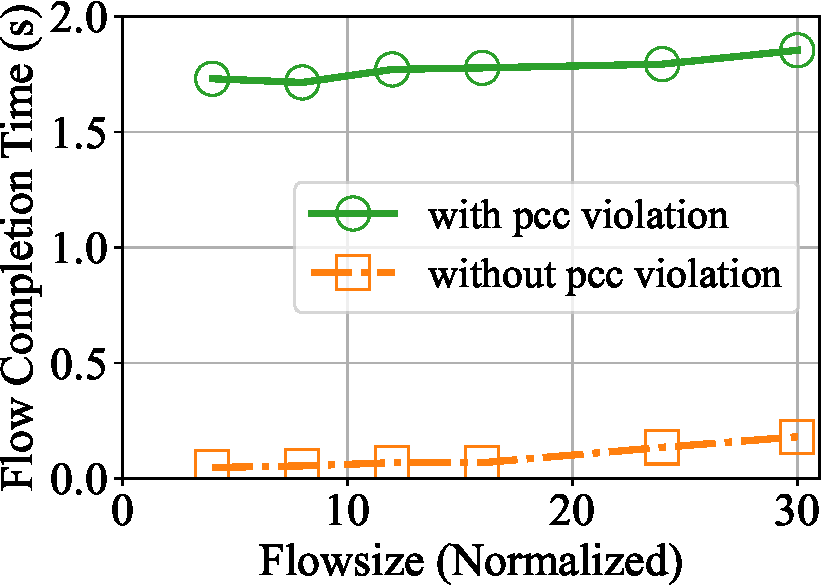
\includegraphics[width=1\textwidth]{experiment/0pccviolation.pdf}
		\caption{The impact of PCC violations.}
		\label{100}
	\end{minipage}%
	\centering
	\begin{minipage}[t]{0.33\linewidth}
		\centering
		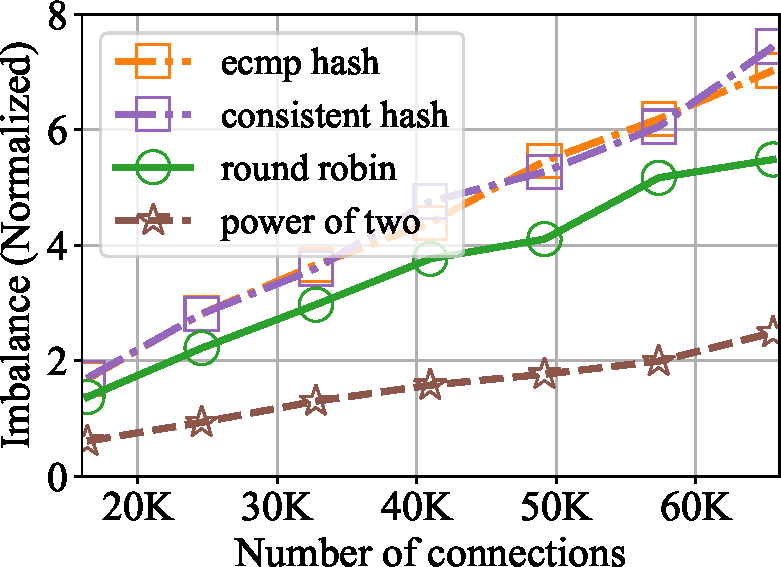
\includegraphics[width=0.977\textwidth]{experiment/1balancescheme.pdf}
		\caption{Load imbalance.}
		\label{2}
	\end{minipage}%
	\begin{minipage}[t]{0.33\linewidth}
		\centering
		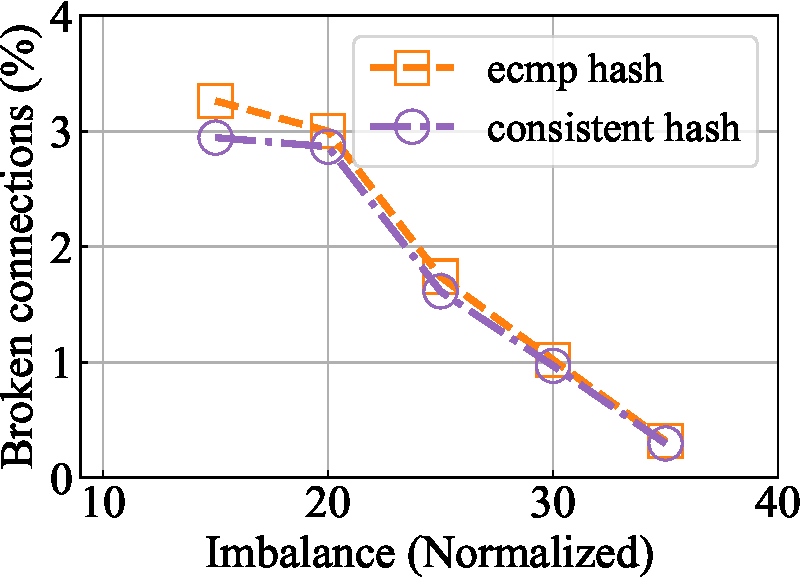
\includegraphics[width=0.988\textwidth]{experiment/2brokenimbalance.pdf}
		\caption{Relationship between broken connections and load imbalance.}
		\label{3}
	\end{minipage}
\end{figure*}

\section{BACKGROUND AND MOTIVATION}
Datacenter operators assign a virtual IP (VIP) address to each service they operate, and this virtual IP address is generally assigned to the L4 LB. Each VIP is associated with a set of servers (DIP pool) providing that service. The purpose of this paper is to design a simple and practical L4 LB scheme that evenly distributes incoming traffic across all available DIPs. In this section, we begin by presenting the advantages and disadvantages of both load-agnostic and load-aware L4 LB. Subsequently, we discuss the design motivation of Maat.
\subsection{Previous work}
\textbf{Load-agnostic L4 LB:}
Load-agnostic load balancers are characterized by relying on simple hash calculations\footnote{Hash algorithms refer to algorithms such as ECMP, consistent hashing, and minimum perfect hashing.} to distribute incoming traffic among backend servers. Since these LBs do not consider the current load status of the servers, they often result in load imbalances. Research has shown that hash-based methods can suffer up to 30\% load imbalance \cite{eisenbud2016maglev}.

Ananta \cite{patel2013ananta} is a L4 LB that relies on ECMP to forward traffic. Due to its slow packet processing speed, Duet \cite{gandhi2014duet} offloads part of the workload to the switch to alleviate the performance bottleneck that exists in Ananta. Silkroad \cite{miao2017silkroad} use programmable switches to further improve throughput, but these solutions all use ECMP to forward traffic, and PCC violations are prone to occur when the DIP pool updates. Google proposes Maglev \cite{eisenbud2016maglev} to effectively alleviate this problem through consistent hashing. Later, Faild \cite{araujo2018balancing} and Beamer \cite{olteanu2018stateless} also adopt consistent hashing as a load balancing scheduling method.

However, consistent hashing may introduce false hits during connection lookups due to the use of digests rather than complete state information. The occurrence of false hits may cause the L4 LB to forward packets to the wrong DIP, resulting in PCC violations. To address these problems, some works proposed applying Othello hashing to L4 LB \cite{yu2018memory}. For instance, Concury \cite{shi2020concury} and SDLB \cite{yu2017sdlb} are designed for cloud data centers and mobile edge computing, respectively. Due to the false-hit freedom characteristics of this hash algorithm, L4 LB can fully maintain PCC. Although load-agnostic LBs have made great progress in maintaining PCC. However, fairness as a first-class citizen in L4 LB has not received enough attention, and some schemes even ensure PCC at the expense of fairness.

\textbf{Load-aware L4 LB:}
Research in recent years has also realized that it is wrong for load-agnostic load balancers to sacrifice fairness to maintain PCC \cite{zhang2020fast, barbette2021cheetah, yao2022hlb}. As a result, some works have begun to strive to enhance fairness while maintaining PCC. The mainstream method is to adjust the weight of different servers through real-time network status (e.g., server status, traffic status), so that incoming traffic has a greater probability of selecting a more suitable server, thereby alleviating the load imbalance based on the hash scheme.

Server status-based methods collect information such as CPU and memory usage to guide forwarding strategies. However, they face three main challenges: 1) This type of solution is difficult to cope with the challenge of device heterogeneity and can easily cause L4 LB to make wrong forwarding decisions, thus damaging fairness \cite{zhang2020fast}. Here, device heterogeneity \cite{abdelmoniem2021towards} refers to the presence of multiple different devices within the same service. For server operators, a single service may be provided by multiple machines of various models \cite{sharma2011modeling}. Moreover, with the rise of cloud computing \cite{garg2014sla} and network function virtualization (NFV) \cite{lin2017enabling}, the device heterogeneity faced by contemporary cloud data centers may be more complex. 2) Server status-based solutions usually require additional high-performance equipment to implement complex interactions between LB and servers. For example, Spotlight \cite{aghdai2020spotlight} requires specifying an additional server (Intel i9 7900x with 64 GB RAM) as a dedicated controller for traffic management. 3) These methods also introduce security risks due to the frequent interactions required between the L4 LBs and servers to obtain accurate, real-time status updates. Third-party attackers can easily use sniffing attacks \cite{xiao2015detecting} to obtain server status information from frequent interactions, thereby conducting more targeted DDoS attacks \cite{garber2000denial}, causing some servers to go down or even the entire service to collapse. In summary, server state-based solutions not only face huge scalability challenges but also have difficulty handling potential security issues.

Another approach involves the load balancer directly collecting traffic status, which avoids complex interactions with servers, addresses potential security issues, and provides good scalability. However, there are also some problems with traffic state-based methods. For example, in LBAS \cite{zhang2020fast}, the scheduling policy relies on the number of active connections on the current server, ignoring the different effects of flow size on server load. Therefore, this approach runs the risk of forwarding incoming traffic to inappropriate servers. Although some methods \cite{guo2022libra} are aware of this problem, they still use a coarse-grained approach to collect traffic status information, which also leaves room for improper traffic allocation. To solve these problems, Maat introduces a more fine-grained traffic statistics method. With packet-level traffic statistics, incoming traffic can be assigned more accurate servers for better fairness.


\subsection{Motivation}
\textbf{PCC violations significantly increase the tail latency.} Maintaining PCC in L4 LB is crucial, as our experiments demonstrate that it has a significant impact on performance. We deploy HTTP service on three servers (1 client, 2 servers) and use a Tofino switch as the L4 LB. During this experiment, we generate workloads with increasing flow sizes and perform DIP pool updates. The experimental results in Fig. \ref{100} show that the FCTs with PCC violations are 10.28 times higher than those without PCC violations. This indicates that PCC violations severely affect the processing of incoming traffic, especially latency-sensitive traffic, potentially leading to unacceptable service level agreement (SLA) violations. From the experiment, it is clear that maintaining PCC is a prerequisite for L4 LB to improve fairness. However, we must ensure that load balance is not sacrificed to maintain PCC \cite{barbette2020high}.

\textbf{Hash-based L4 LB cannot spread incoming traffic evenly.} We compare ecmp/consistent hashing and other scheduling strategies for their ability to evenly distribute incoming traffic. The workload is generated based on the traffic distribution of Web search \cite{alizadeh2010data}. The experimental results are shown in Fig. \ref{2}. Among the four commonly used strategies, the power of two choices exhibits significant advantages. Specifically, it performs 2.83 times better than ecmp/consistent hashing and 2.21 times better than round-robin. However, the limitations of maintaining PCC make it challenging to directly implement methods like the power of two choices or round-robin in L4 LB environments. Cheetah proposed a method that requires modifying the TCP/IP protocol stack by encoding the selected server’s identifier into a cookie added to all the packet headers.

\textbf{Hash-based L4 LB cannot guarantee PCC and load balance at the same time.} We conduct a simple experiment to evaluate whether these hash-based L4 LB can simultaneously achieve the two goals of enhancing fairness and maintaining PCC. In this experiment, we use an imbalance threshold as input and removed/added the server from the DIP pool when the server load is above/below the threshold \cite{barbette2021cheetah}. We use the traffic distribution of Web search to generate 100K connections. Fig. \ref{3} illustrates the relationship between fairness and the ratio of broken connections. It is worth noting that even when the load imbalance (normalized) reaches 30, the ratio of broken connections remains around 1\%. This demonstrates that L4 LB faces a conflict between enhancing fairness and ensuring PCC. In existing hash-based schemes, a common approach is to sacrifice load balance \cite{eisenbud2016maglev, olteanu2018stateless}, which goes against the original purpose of load balancing.

In brief, these experiments demonstrate that existing schemes cannot meet the three requirements of L4 LB (fairness, PCC, scalability). This motivates us to propose a new L4 LB scheme.


\subsection{Background algorithms}
\textbf{Power of two choices} is a commonly used scheduling method in load balancing, and in Figure \ref{3} we can see that it can achieve better fairness. This algorithm, originally proposed by David G. Andersen and Michael Kaminsky \cite{mitzenmacher2001power}, significantly enhances load balancing performance in supermarket models with a single input queue and multiple output queues using a limited number of choices (e.g., d = 2) \cite{ghorbani2017drill}.

However, in L4 LB, two random choices make maintaining the mapping between connections and servers more complex \cite{zhang2021loom, barbette2020high}. Therefore, most existing solutions still use hash functions to select servers because the hash function helps mitigate PCC violations. Unlike the existing L4 LB, Maat uses a novel scheduling method inspired by the power of two choices termed the power of one random choice. The basic idea is to compare the load of one hash selected server and one randomly selected server and choose the one with less load to forward traffic. 


\textbf{Othello hashing} is a minimal perfect hashing algorithm \cite{yu2017othello, chazelle2004bloomier} that supports forwarding information base and load balancing in programmable networks, including two arrays as its data plane, and a construction program in its control plane, as the interaction protocols of the two planes \cite{shi2020concury}. Since the Othello hashing has the characteristics of fast query speed and no false hits \cite{yu2017sdlb}, which can help us maintain PCC. So we use it as the hash function of the power of one random choice. We use the example in Fig. \ref{4} to demonstrate the operation of constructing and querying Othello.

Construction in the Othello control plane.
In Fig. \ref{4}, two arrays \emph{A} and \emph{B} are constructed with \emph{$m_a$} and \emph{$m_b$} elements, respectively. Each array element is an \emph{l}-bit value. In this example, \emph{l} = 2 and assume \emph{$m_a$} = \emph{$m_b$} = 5 for better illustration. For each value \emph{i} in \emph{A} we place a vertex \emph{$a_i$}, and for each value \emph{j} in B we place a vertex \emph{$b_j$}. Two hash functions \emph{$h_a$} and \emph{$h_b$} are used to compute the hash values of all \emph{$f_i$}. Then, for each \emph{$f_i$}, we place an edge between the two vertices corresponding to its hash value. For example, \emph{$h_a(f_{\text{2}})$} = 3 and \emph{$h_b(f_{\text{2}})$} = 1, so place an edge connecting \emph{$a_3$} and \emph{$b_1$}. For a \emph{$f_i$} and its corresponding \emph{index}, Othello hashing requires that two connected elements $\emph{A}[\emph{$h_a(f_{\text{i}})$}] \oplus \emph{B}[\emph{$h_b(f_{\text{i}})$}] = \emph{index}$, where $\oplus$ is a bitwise exclusive OR (XOR). For \emph{$f_2$} in this example, \emph{$a_3$} $\oplus$ \emph{$b_1$} = $11_2$ = 3. Note that after placing the edges of all \emph{$f_i$}, the bipartite graph formed by all vertexes must be acyclic. If a cycle is found, the construction must find another pair of hash functions to reconstruct the bipartite graph. It has been proved that the expected time cost of constructing a bipartite graph with \emph{n} \emph{$f_i$} is O(\emph{n}) \cite{yu2018memory}.

Query in the Othello data plane.
The Othello query structure contains two arrays \emph{A} and \emph{B}, as shown in Fig. \ref{4}. To query the value of \emph{\emph{$f_{\text{1}}$}}, we need to compute \emph{$h_a$} and \emph{$h_b$}, which are mapped to \emph{$a_1$} of \emph{A} and \emph{$b_0$} of \emph{B}. We then compute the bit-wise XOR of two vertexes and get the \emph{index} is $00_2$. For each packet, only two memory accesses are required, that is, reading a value from arrays \emph{A} and \emph{B} respectively, which can achieve fast queries.

\begin{figure}[t]
	\setlength{\abovecaptionskip}{0pt}
	\setlength{\belowcaptionskip}{-10pt}
	\centering
	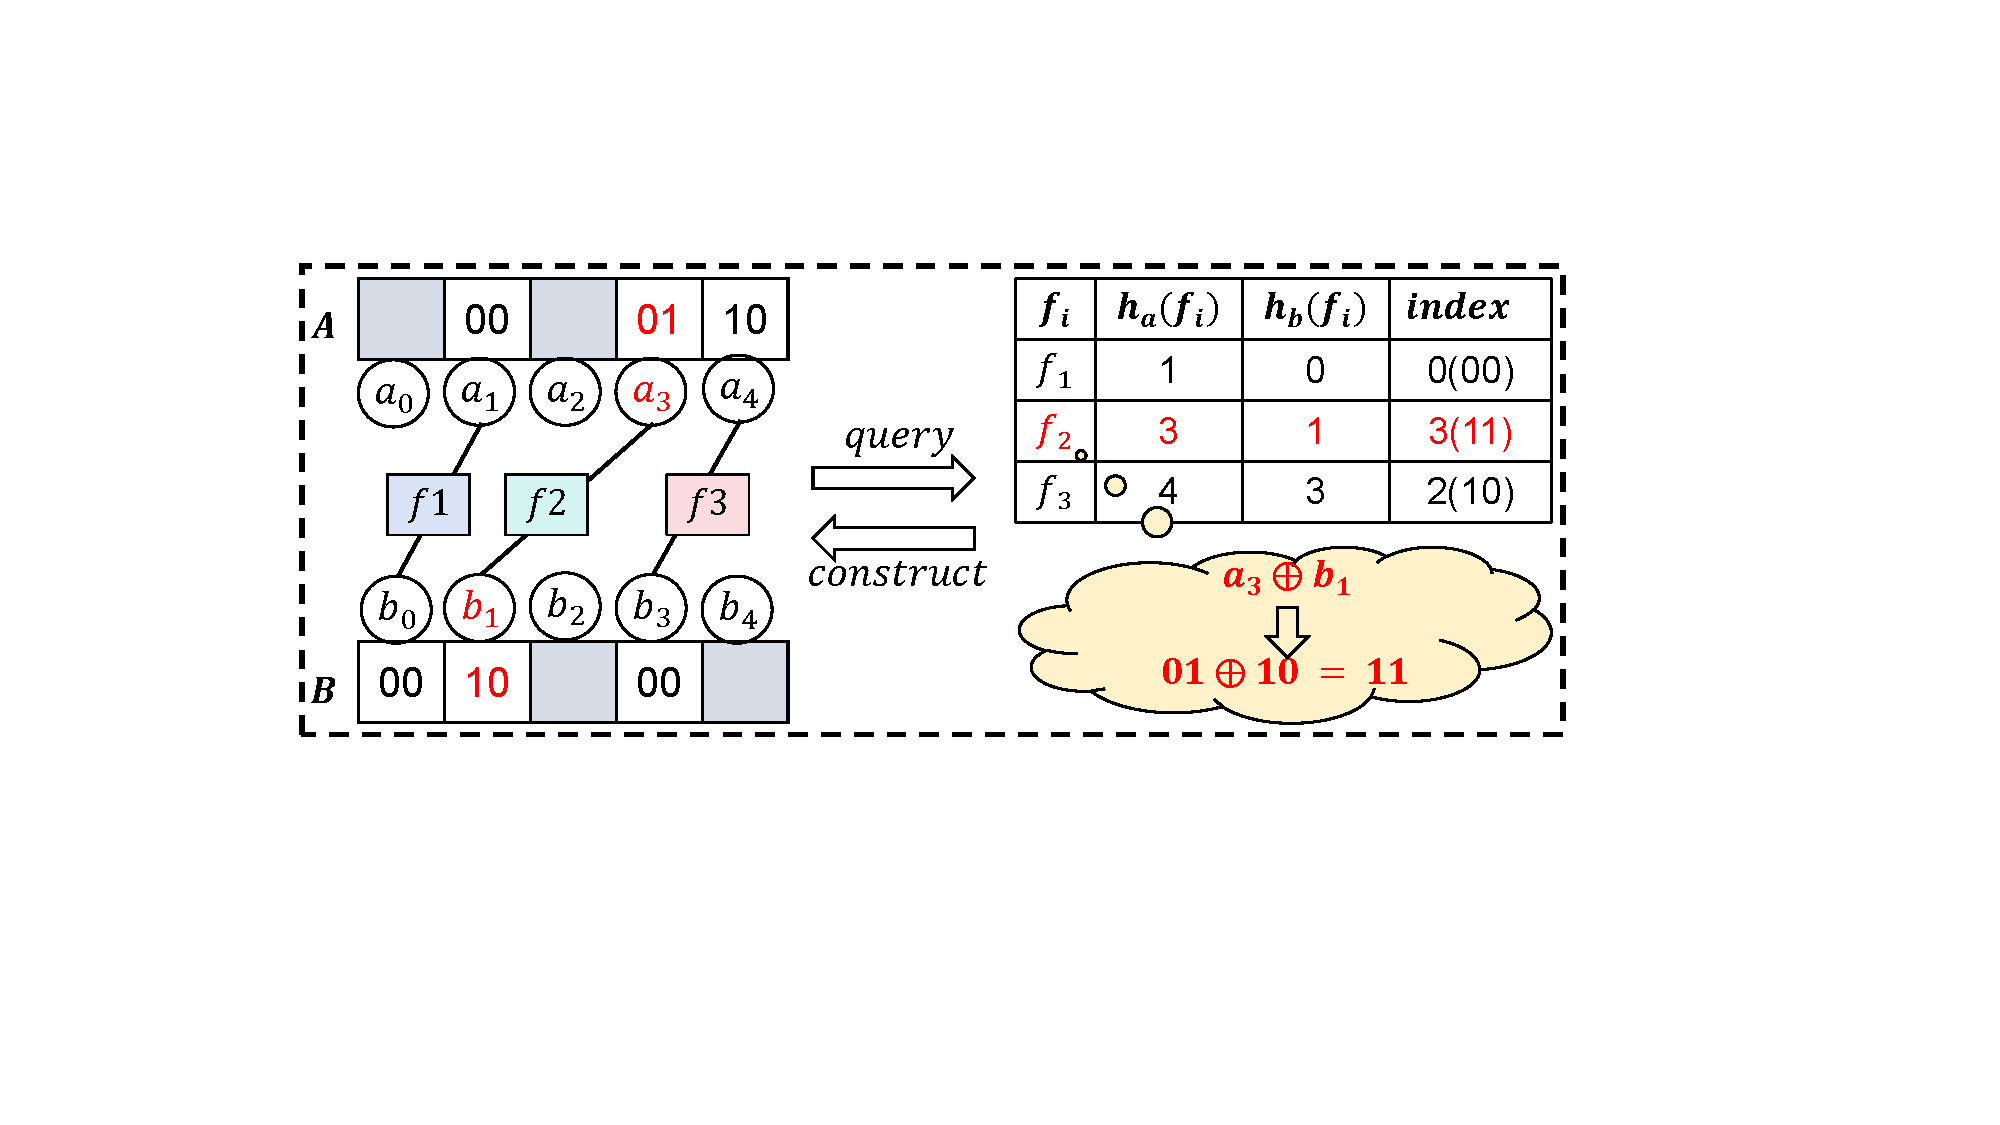
\includegraphics[width=1\linewidth]{figure/othello.pdf}
	\caption{The construction and query of Othello structure. \emph{$h_a$} and \emph{$h_b$} are the hash functions corresponding to the arrays \emph{A} and \emph{B} respectively.}
	\label{4}
\end{figure}